\documentclass{beamer}

\mode<presentation> {
\usetheme{Madrid}
%\usecolortheme{dolphin}
%\usecolortheme{lily}
%\usecolortheme{seahorse}
\setbeamertemplate{caption}[numbered]
\setbeamerfont{caption}{size=\scriptsize}
\setbeamertemplate{navigation symbols}{} % To remove the navigation symbols from the bottom of all slides uncomment this line
}

\usepackage{graphicx}
\usepackage{booktabs}
\usepackage{pifont}
\usepackage{threeparttable}
\usepackage{longtable}
\usepackage{booktabs}
\usepackage{multirow}
\usepackage{amsmath}
\usepackage{float}
\usepackage{array}
\usepackage{subfigure}
\usepackage{bbm}
\usepackage{comment}
\usepackage{adjustbox}
\usepackage{lscape}
\usepackage{hyperref}
\usepackage{setspace}
\usepackage{appendixnumberbeamer}
\usepackage{booktabs}
\usepackage{tabulary}
\usepackage{multirow}
\usepackage{multicol}

\newcolumntype{x}[1]{>{\centering\arraybackslash\hspace{0pt}}p{#1}}

%----------------------------------------------------------------------------------------
%	TITLE PAGE
%----------------------------------------------------------------------------------------

\title[Decompr]{An application of Decompr}
\author[Kummritz (WTO), Quast (UNCTAD)]{Victor Kummritz (WTO) \and Bastiaan Quast (UNCTAD)} 
\institute[] 
{
{\normalsize WTO}
\vspace{-0.5cm}
}
\date{03/03/17}
\begin{document}

\begin{frame}
\titlepage % Print the title page as the first slide
\end{frame}

%\begin{frame}
%\frametitle{Overview} % Table of contents slide, comment this block out to remove it
%\tableofcontents % Throughout your presentation, if you choose to use \section{} and \subsection{} commands, these will automatically be printed on this slide as an overview of your presentation
%\end{frame}

%----------------------------------------------------------------------------------------
%	PRESENTATION SLIDES
%----------------------------------------------------------------------------------------

%------------------------------------------------

\begin{frame}

\frametitle{Background}

\begin{itemize}
\item Advanced GVC indicators are based on complex matrix manipulations.\\
\item[$\rightarrow$] Develop a new tool, the R package $decompr$, to derive a wide set of detailed GVC indicators based on decompositions proposed by Hummels et al. (2001), Wang et al. (2013, henceforth WWZ), and Koopman et al. (2014).\\\
\item Many analyses of GVC integration patterns are based on a limited set of countries or indicators.\\
\item[$\rightarrow$] Apply $decompr$ to the new OECD Input-Output tables (ICIOs) with extensive country coverage to reveal novel stylized facts in the GVC integration patterns of developing economies.\\\
\end{itemize}

\end{frame}

%------------------------------------------------

\begin{frame}

\frametitle{Indicators}

Standard indicators based on Hummels et al. (2001):
\begin{itemize}
\item $fvax$ - foreign value added in exports (Backward linkages, Vertical Specialisation, Inverse VAX ratio, i2e).\\
\item $dvar$ - domestic value added in re-exports (Forward linkages, Vertical Specialisation 1, e2r).\\\
\end{itemize}

Advanced indicators based on WWZ and Koopman et al. (2014):
\begin{itemize}
\item $dva\_fin$ ($fva\_fin$) - domestic (foreign) value added in final good exports.\\
\item $dva\_inter$ ($fva\_inter$) - domestic (foreign) value added in intermediate good exports.\\
\item $rdv$ - returned domestic value added.\\\
\end{itemize}

\end{frame}

%------------------------------------------------

\begin{frame}

\frametitle{Findings}

\begin{itemize}
\item We confirm the \textbf{rapid expansion of GVCs from 1995 to 2011} and show that by 2011 GVCs already reached their pre-crisis level.\\\
\item We show, using novel indicators by WWZ, that GVCs have become longer over time.
\end{itemize}

\end{frame}

%------------------------------------------------

\begin{frame}

\frametitle{Findings}

Interestingly, these trends are increasingly \textbf{driven by developing economies}.
\begin{figure}[h]
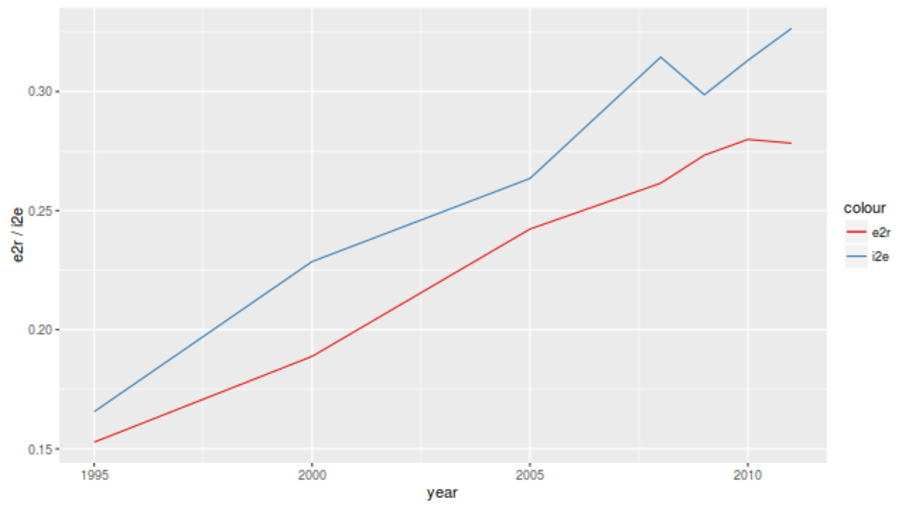
\includegraphics[width=0.9\textwidth]{Dev_Share.pdf}
\caption{Developing countries' share in global backward ($i2e$) and forward ($e2r$) linkages}
\end{figure}

\end{frame}

%------------------------------------------------

\begin{frame}

\frametitle{Findings}

GVC integration \textbf{patterns of developing countries differ from advanced countries' patterns} once advanced indicators are considered.
\begin{table}[htbp]\scriptsize
  \centering
  \caption{WWZ decomposition results by income group}
    \begin{tabular}{l|ccccc}
    \toprule
     \hline
    Country group & $fva\_fin$ & $fva\_inter$ & $dva\_fin$ & $dva\_inter$ & $rdv$ \\
     \hline
   Developing & 42.07\% & 57.93\% & 44.09\% & 54.73\% & 1.18\% \\
    High-income  & 39.38\% & 60.62\% & 40.73\% & 56.85\% & 2.42\% \\
         \hline
    \bottomrule
    \end{tabular}
\end{table}

\end{frame}

%------------------------------------------------

\begin{frame}

\frametitle{Findings}

However, there is convergence in patterns.
\begin{figure}[h]
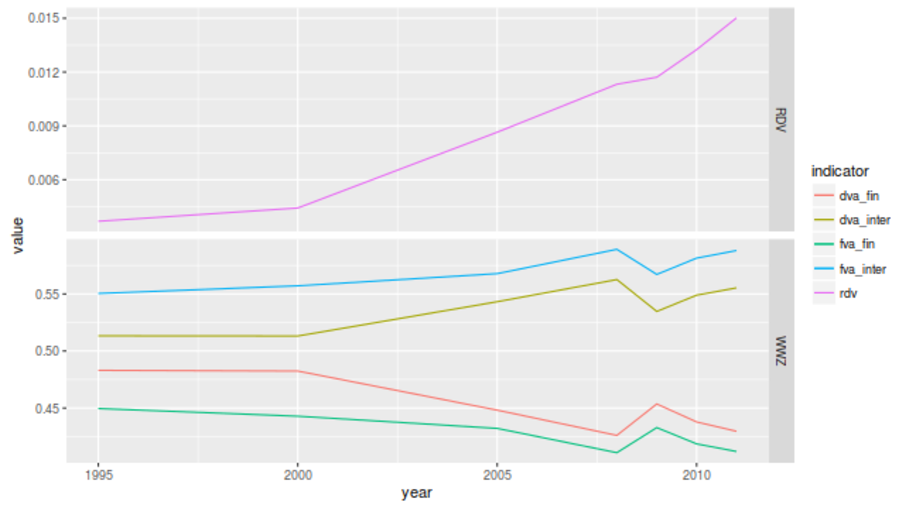
\includegraphics[width=0.9\textwidth]{wwzchange.pdf}
\caption{Development of developing economies� WWZ indicators over time}
\end{figure}

\end{frame}

%------------------------------------------------

\begin{frame}

\frametitle{Findings}

We observe considerable heterogeneity among developing economies.
\begin{table}[htbp]\scriptsize
  \centering
  \caption{WWZ decomposition for selected developing economies}
    \begin{tabular}{l|ccccc}
    \toprule
     \hline
    Country group & $fva\_fin$ & $fva\_inter$ & $dva\_fin$ & $dva\_inter$ & $rdv$ \\
     \hline
   Malaysia & 39.3\% & 60.7\% & 40.8\% & 58.9\% & 0.4\% \\
    Argentina  & 51.2\% & 48.9\% & 51.9\% & 47.9\% & 0.2\% \\
         \hline
    \bottomrule
    \end{tabular}
\end{table}

\end{frame}

%------------------------------------------------

\end{document} 